% LaTeX file for resume 

% The value for margin is ignored, but it has to be there or geometry throws
% errors. The margin option causes section titles to appear to the left of body text 
\documentclass[margins]{res-compat} 
%\usepackage[rmargin=1.7in,lmargin=0.3in,vmargin=0.5in]{geometry}
\usepackage{helvetica}
\usepackage{graphicx}
\usepackage{anysize}
\usepackage{hyperref}
\marginsize{0.3in}{1.7in}{0.3in}{0.5in}

\begin{document} 

\name{Russell E. Harmon} % the \\[12pt] adds a blank line after name

\address{{\bf School Address} \\ Rochester Institute of Technology \\ Computer
Science \\ 39 Nathaniel Rochester Hall \\ Rochester, NY 14623}
\address{{\bf Permanent Address} \\ 2710 Avenue J N/W \\ Winter Haven, FL
33881 \\ (863) 514-7014 \\ russ@eatnumber1.com}
 
\begin{resume} 

\section{Technical Skills}
	\begin{itemize} \itemsep -2pt
		\item Cisco switches
		\item UNIX
		\begin{itemize} \itemsep -2pt
			\item Linux
			\item Solaris
			\item BSD
		\end{itemize}
		\item Java
		\item C
		\item C++
		\item Python
		\item PC troubleshooting and repair
	 \end{itemize}

\section{Education}
	\begin{itemize} \itemsep -2pt
		\item Rochester Institute of Technology – Computer Science, minor in Music.
		\item Herbert H. Lehman High School - College Prep Program
		\begin{itemize} \itemsep -2pt
			\item AP English
		\end{itemize}
		\item Lehman College - Course work in Q-Basic (age 12)
	\end{itemize}

\section{Experience}
	\begin{itemize} \itemsep -2pt
		\item SafeNet Inc, Belcamp, MD \hfill June 2008 - November 2008
		\\* Engineering Intern \hfill http://www.safenet-inc.com
		\begin{itemize} \itemsep -2pt
			\item Work as a developer on a team of 7 on SMCII (the SafeNet
			Management Console).
			\item Java development with JBoss, Hibernate and JSF
		\end{itemize}
		\item New York City Department of Education, Bronx, NY \hfill September 2002 - June 2006
		\\* IT Specialist \hfill http://schools.nyc.gov
		\begin{itemize} \itemsep -2pt
			\item Setup and maintain computer systems throughout Lehman High School
			\item Diagnose, repair, and maintain the network
			\item Reformat machines using Norton Ghost
			\item When the school got new machines, I had to migrate user's settings onto the new machines
			\item Diagnose and eliminate viruses and malware on the school's network and computer systems
			\item Audit the network for malicious activity
		\end{itemize}

		\item New York Sailing \& Yacht Club, Bronx, NY \hfill 2001-2005
		\\* Launch Operator \hfill http://www.startsailing.com
		\begin{itemize} \itemsep -2pt
			\item Taxi patrons to their boats moored in the harbor
			\item Experienced in both motor and sail powered small craft operation
		\end{itemize}

		\item City Island Computer Services, Bronx, NY \hfill 1998-1999
		\\* Apprentice (age 10)
	\end{itemize}

\section{Honors and Awards}
	\begin{itemize} \itemsep -2pt
		\item NYC regional robotics award winner – 27th place in the national competition
		\item Honor roll 2003-2005
		\item Visual Basic Programming Award for academic excellence, 2005
		\item First Place Sailing Award 2000, 2002
	\end{itemize}

\section{Special Accomplishments}
	\begin{itemize} \itemsep -2pt
		\item At age 8 built my first computer, at age 12 attended my first programming class at Lehman College.
		\item Designed and implemented an encryption algorithm using a combination of transposition and substitution.
		\item Rocking the Boat – built a boat for needy children from the South Bronx.
	\end{itemize}

\section{Certifications}
	\begin{itemize} \itemsep -2pt
		\item Cisco Academy, with honors (terms 1 and 2)
		\item A+
		\item MOUS (Word)
	\end{itemize}

\end{resume}
\pagebreak[4] % The 4 makes it a VERY INSISTENT requirement for a page break.
\marginsize{-1.5in}{-1.5in}{-0.5in}{-0.5in}
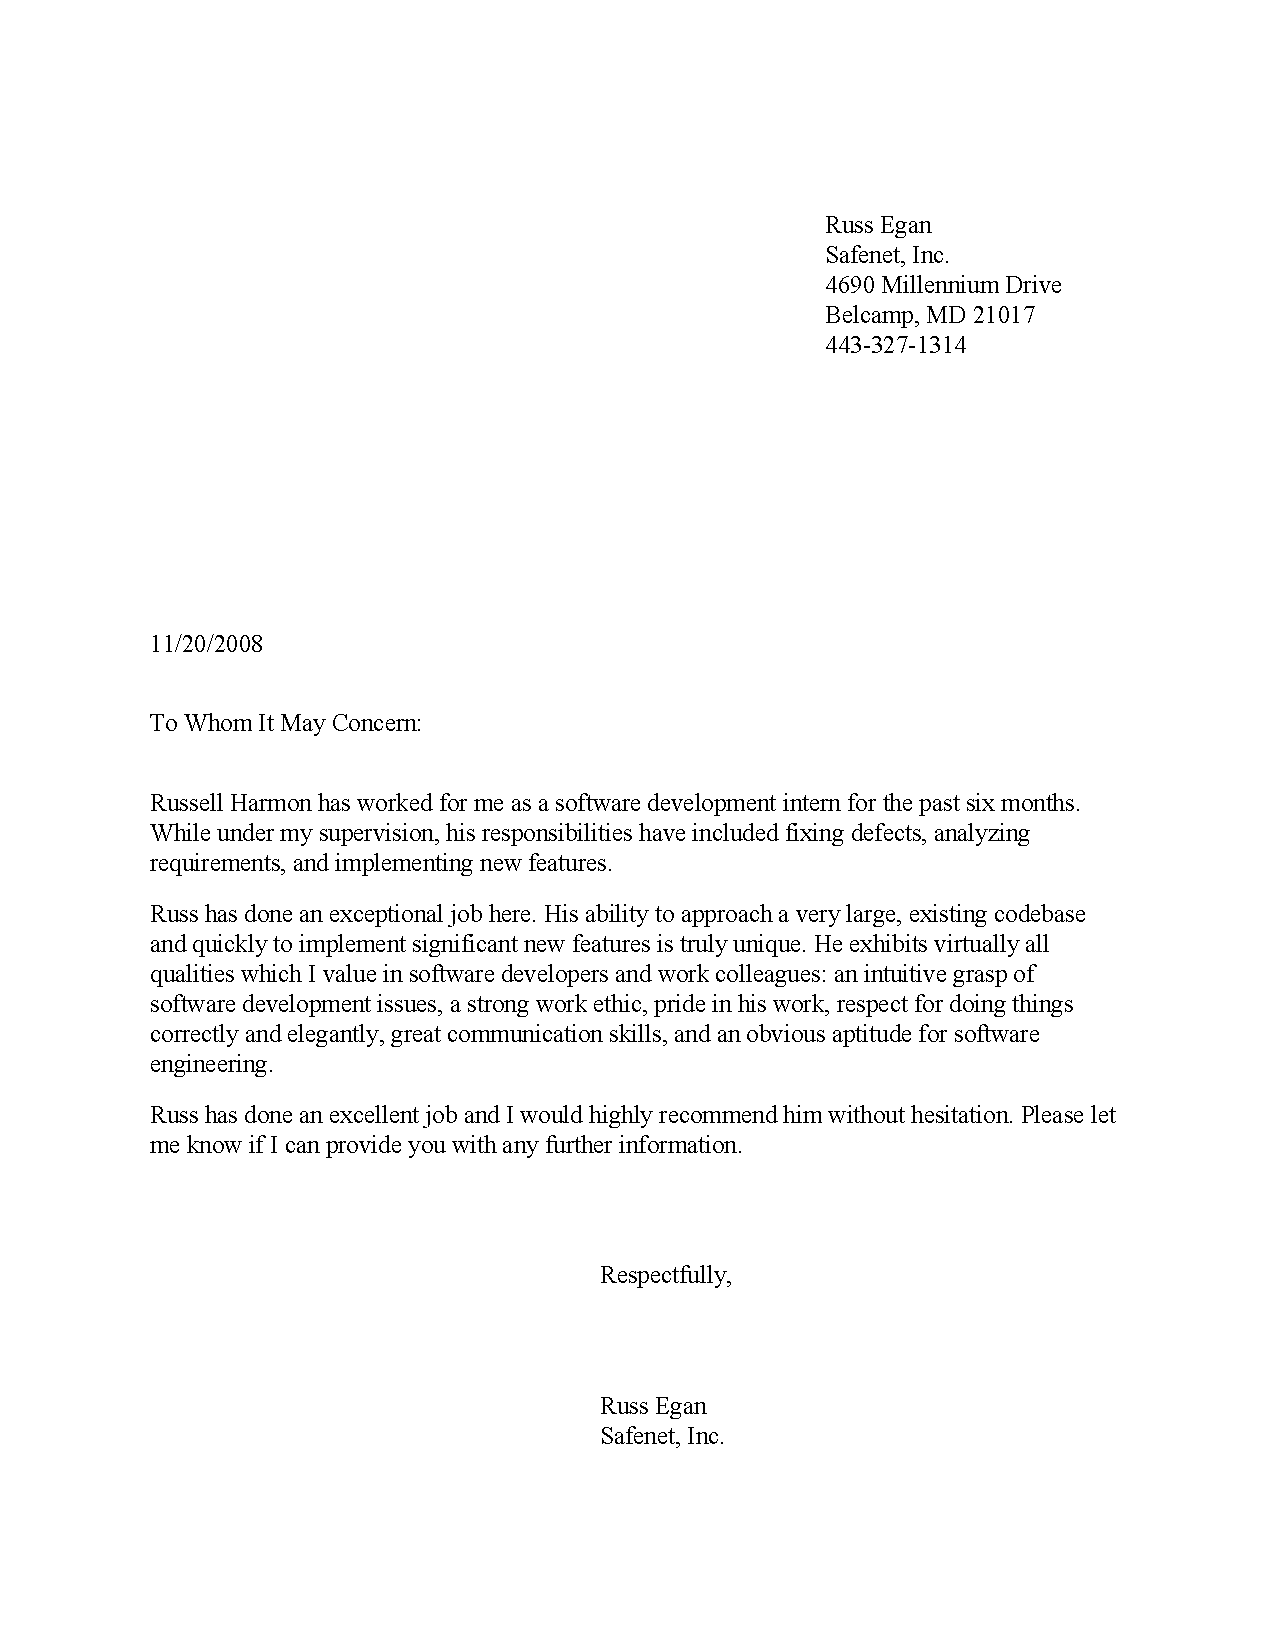
\includegraphics{sfnt-recommendation.pdf}
\end{document}
